%!TEX root = project.tex

\chapter*{About this project}
\paragraph{Abstract}
Data visualisation has become popular, in part due to everyone's experience with the global pandemic Covid-19. Information is delivered in easy to understand visual representations. As this is an emerging area, the team decided to investigate different methods of data visualisation, see which performed the best for different scenarios and to develop a data visualisation application. The main focus of the application is on Covid-19, data is being generated at least daily worldwide for Covid-19. The application includes examples of other pandemics such as SARs, MERs and historic epidemics of smallpox and polio.

\paragraph{Authors}
This project was developed as part of a fifteen credit module by Grace Keane, Jina Kim and Shirin Nagle, fourth year students of Galway Mayo Institute of Technology.

\paragraph{Acknowledgements} The authors would like to acknowledge the time and advice given by the project supervisor Dr. John French.

\chapter{Introduction}
This chapter will serve as a prelude to the project. The context, objectives and metrics for success and failure will be defined, followed by a thorough summary of the project domain and an introduction into each chapter of the dissertation and its relevance.

\section{Context}
During the decision making process the team decided that the project must be relevant as well as interesting. The project must encourage the use of existing skills as well as allow for the natural development of new and relevant techniques and processes while also being worthy of scope.

\vspace{5mm} %5mm vertical space

Data visualisation and analysis techniques have been the front and center in the efforts to communicate the statistics as well as the science around the COVID-19 virus. Interactive dashboards with several charts and graphs surfaced in different formats to offer concise ways to make sense of complex and overwhelming pandemic data sets. These techniques have become essential in informing the general public as well as healthcare providers, scientists and governments of the overall COVID-19 growth. 

\vspace{5mm} %5mm vertical space

As a result, the team felt it would be beneficial as well as informative to create a web application that would take large COVID-19 data sets as well as other epidemic data and create a series of data visualisations from it. As well as compare past and present viruses to distinguish similarities along with differences. This would provide a clear view of COVID-19 and how similar viruses have spread.



\vspace{5mm} %5mm vertical space

Once the project area had been decided on, each team member focused on a pandemic or epidemic, investigated where to source relevant information for the pandemic or epidemic, and investigated different technologies for displaying data in a visual manner.

\begin{itemize}
\item Provide a context for your project.
\item Set out the objectives of the project
\item Briefly list each chapter / section and provide a 1-2 line description of what each section contains.
\item https://github.com/4th-year-project-2020-2021/Final-Year-Project-Data-Visualization.
\\provide a brief list of the main elements at the URL.
\end{itemize}

\section{Project Objectives}
As previously mentioned, the end goal of the project is to create a web application that would process different virus data and create various data visualisations to ensure a simple way for users to view large complex pandemic data. To ensure the end goal was reached, the team outlined objectives to be followed throughout development.

\begin{itemize}
  \item Investigate the field of interest and scope for the project.
  \item Evaluate and research the appropriate frameworks and tools available for development.
  \item Incorporate state of the art technologies, frameworks, databases and tools that will allow users to view, add, update, delete, post and retrieve data.
  \item The web application will, at a minimum allow users to sign-up, login, view data visualizations as well as incorporate user interaction features, create unique user visuals and post user data to databases. 
\end{itemize}

\subsection{Metrics for Success and Failure}
The outlining criteria for success and failure were important in ensuring the project remained on track throughout development and therefore allow the project to achieve the outlined goals in a timely and standard-driven manner. The defined metrics are of similar nature to that of the underlying objectives defined in \emph{Section.....} but explained in a higher level.

\vspace{5mm} %5mm vertical space

\subsection{Applied Project}
A selection of metrics were outlined specifically for the dissertation, they are as follows.

\begin{itemize}

    \item \emph{The final dissertation should be easily understood, allowing readers without knowledge or familiarity of the subject area to form a suitable understanding of the concept and areas discussed.} In order to accurately measure this metric, input was received from family and fellow students, who would kindly read newly integrated sections and provide useful feedback.

    \item \emph{The  dissertation should be in order of 30,000 - 45,000 words, excluding appendices as well as approximately 105 pages (excluding diagrams, abstract, TOCs, references, appendices etc.)}
    
\end{itemize}

\section{Applied Project}
A selection of metrics were outlined specifically for the development of the applied project, they were as follows.

\begin{itemize}

    \item \emph{The applied project must be easy to use, navigate and attempt to deal with a task of problem deemed to be of sufficient technical challenge and depth.} To ensure this was adhered to, at frequent stages of development feedback from fellow students and Dr. John French was considered and documented relating to the application.

    \item \emph{Collaboration between team members and supervisor should be consistent to ensure a smooth work flow throughout the project planning and development.)} In order for this metric to be adhered to the team maintained communication as well as with the supervisor throughout the development and planning of the applied project.
    
\end{itemize}

\section{Dissertation Summary}
This section will contain a brief overview of the dissertation structure and will provide a short description of each chapters objectives.

\section{Methodology}
In this chapter, the processes undertaken during the life cycle of the project regarding planning, testing and development will be outlined. Investigating development methods and methods employed during the research phase, their results and the effect they had on the direction of the project will be brought to the attention of the reader. Additional, the decisions, thought process and influential factors leading up to those processes and design implementations will also be described.

\section{Technology Review}
A technological review will encapsulate the technical aspect of the project. This includes the different technologies incorporated, their implementation, their roll, and why they were chosen. The benefits of the chosen technologies will be critically analysed and compared with similar alternatives. 

\section{System Design}
A detailed explanation of the overall system architecture will be provided. Diagrams will be included to help illustrate and explain the inner workings of the application at a high level.

\section{System Evaluation}
An evaluation of the final applied project against the initial project objectives. The final result of the project will be critically analysed including an analysis of areas of software quality, improvements or changes to the overall project.

\section{Conclusion}
To conclude, a brief summary of the context and objectives to remind the reader about the overall rationale and goals of the project. Key insights will be identified and reflected on. A final analysis will describe the teams overall experience and what the team learned while working on a project similar to one encountered in the software industry. 








\chapter{Methodology}
About one to two pages.
Describe the way you went about your project:
\begin{itemize}
\item Agile / incremental and iterative approach to development. Planning, meetings.
\item What about validation and testing? Junit or some other framework.
\item If team based, did you use GitHub during the development process.
\item Selection criteria for algorithms, languages, platforms and technolo-gies.
\end{itemize}
Check out the nice graphs in Figure \ref{tikz:graphs}, and the nice diagram in Figure \ref{tikz:mydiagram}.

\begin{figure}
  \centering
  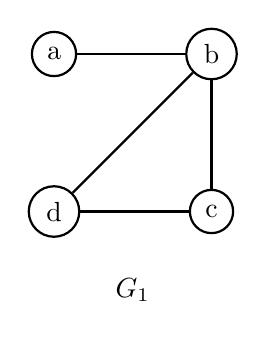
\begin{tikzpicture}
  \begin{scope}[every node/.style={circle,thick,draw}]
  \node (a) at (0,2) {a};
  \node (b) at (2,2) {b};
  \node (c) at (2,0) {c};
  \node (d) at (0,0) {d};
  \end{scope}
  \begin{scope}[every edge/.style={draw=black,thick}]
  \path (a) edge (b);
  \path (b) edge (c);
  \path (b) edge (d);
  \path (c) edge (d);
  \end{scope}
  \node () at (1,-1) {$G_1$};
  \end{tikzpicture}
  \hspace{1.5cm}
  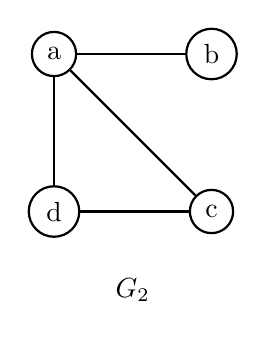
\begin{tikzpicture}
  \begin{scope}[every node/.style={circle,thick,draw}]
  \node (1) at (0,2) {a};
  \node (2) at (2,2) {b};
  \node (3) at (2,0) {c};
  \node (4) at (0,0) {d};
  \end{scope}
  \begin{scope}[every edge/.style={draw=black,thick}]
  \path (1) edge (2);
  \path (1) edge (3);
  \path (1) edge (4);
  \path (3) edge (4);
  \end{scope}
  \node () at (1,-1) {$G_2$};
  \end{tikzpicture}
  \caption{Nice pictures}
  \label{tikz:graphs}
\end{figure}


\begin{figure}
  \centering
  \begin{tikzpicture}[node distance=6cm]
  \node (a) [rect] {A Big Blue Block};
  \node (b) [oval, right of=a] {And His Oval Friend};
  \draw [line] (a) -- (b);
  \end{tikzpicture}
  \caption{Nice pictures}
  \label{tikz:graphs}
\end{figure}


\chapter{Technology Review}
About seven to ten pages.
\begin{itemize}
\item Describe each of the technologies you used at a conceptual level. Standards, Database Model (e.g. MongoDB, CouchDB), XMl, WSDL, JSON, JAXP.
\item Use references (IEEE format, e.g. [1]), Books, Papers, URLs (timestamp) – sources should be authoritative. 
\end{itemize}

\section{XML}
Here's some nicely formatted XML:
\begin{minted}{xml}
<this>
  <looks lookswhat="good">
    Good
  </looks>
</this>
\end{minted}

\chapter{System Design}
FReMP stack is a very powerful and highly scalable stack which reduces complexity of back-end code, deals with the database requests very quickly and brings a user friendly interface for front-end users.

\begin{center}    
      
\includegraphics{img/fremp.PNG}
\end{center}

\begin{itemize}
\item Flask
\item React.js
\item MongoDB Atlas
\item Python

These technologies were chosen as they give developers the ability to handle huge volume of data and, at the same time, render a nice modern interface on the client side. 
\item Architecture, UML etc. An overview of the different components of the system. Diagrams etc… Screen shots etc.
\end{itemize}

\begin{table}[h]
  \centering
  \begin{tabular}{x{2cm}p{3cm}}
    \toprule \\
    Column 1 & Column 2 \\
    \midrule \\
    Rows 2.1 & Row 2.2 \\
    \bottomrule
  \end{tabular}
  \caption{A table.}
  \label{table:mytable}
\end{table}

\chapter{System Evaluation}
As many pages as needed.
\begin{itemize}
\item Prove that your software is robust. How? Testing etc. 
\item Use performance benchmarks (space and time) if algorithmic.
\item Measure the outcomes / outputs of your system / software against the objectives from the Introduction.
\item Highlight any limitations or opportuni-ties in your approach or technologies used.
\end{itemize}

\chapter{Conclusion}
About three pages.

\begin{itemize}
\item Briefly summarise your context and ob-jectives (a few lines).
\item Highlight your findings from the evalua-tion section / chapter and any opportuni-ties identified.
\end{itemize}

